\section{Результаты}

Примерное время работы программы:
\begin{itemize}
    \item[—] Для набора Ling Spam — около 1 часа;
    \item[—] Для набора Spam Assasin — около 3 часов;
    \item[—] Для набора Enron — около 9 часов.
\end{itemize}

Полученные в результате выполнения программы метрические данные приведены в Таблице \ref{table2}. 

\begin{table}[!ht]
    \centering
    \caption{Результаты эксперимента}
    \begin{tabular}{|p{0.13\textwidth}|p{0.18\textwidth}|p{0.13\textwidth}|p{0.13\textwidth}|p{0.13\textwidth}|p{0.13\textwidth}|}
    \hline
        Алгоритм & Данные & Accuracy & Precision & Recall & F1-score \\ \hline
        AO & Ling Spam & 99.17\% & 100.00\% & 95.73\% & 97.58\% \\ \hline
        HGS & Ling Spam & 99.31\% & 100.00\% & 96.09\% & 97.75\% \\ \hline
        SSA & Ling Spam & 87.71\% & 98.94\% & 40.05\% & 41.26\% \\ \hline
        MRFO & Ling Spam & 99.31\% & 100.00\% & 96.22\% & 97.88\% \\ \hline
        RSCV & Ling Spam & 99.03\% & 100.00\% & 94.96\% & 97.16\% \\ \hline
        DEFAULT & Ling Spam & 99.31\% & 100.00\% & 95.85\% & 97.79\% \\ \hline
        AO & Spam Assasin & 97.99\% & 99.11\% & 92.97\% & 95.96\% \\ \hline
        HGS & Spam Assasin & 98.03\% & 99.14\% & 93.19\% & 96.06\% \\ \hline
        SSA & Spam Assasin & 75.73\% & 30.94\% & 42.93\% & 41.97\% \\ \hline
        MRFO & Spam Assasin & 98.03\% & 99.12\% & 93.36\% & 96.07\% \\ \hline
        RSCV & Spam Assasin & 97.84\% & 99.00\% & 92.50\% & 95.67\% \\ \hline
        DEFAULT & Spam Assasin & 97.99\% & 99.08\% & 93.11\% & 95.98\% \\ \hline
        AO & Enron & 98.87\% & 98.14\% & 99.68\% & 98.89\% \\ \hline
        HGS & Enron & 98.88\% & 98.13\% & 99.67\% & 98.90\% \\ \hline
        SSA & Enron & 80.93\% & 92.07\% & 99.83\% & 84.10\% \\ \hline
        MRFO & Enron & 98.88\% & 98.14\% & 99.70\% & 98.91\% \\ \hline
        RSCV & Enron & 98.80\% & 98.02\% & 99.72\% & 98.82\% \\ \hline
        DEFAULT & Enron & 98.86\% & 98.13\% & 99.67\% & 98.89\% \\ \hline
    \end{tabular}
    \label{table2}
\end{table}

Также на основе полученных результатов построены диаграммы $Accuracy$ — на Рисунке 
\ref{AccuracyScheme} и $F1-score$ — на Рисунке \ref{F1Scheme} для возможных сочетаний 
наборов данных и алгоритмов оптимизации.

\begin{figure}[H]
    \centering
    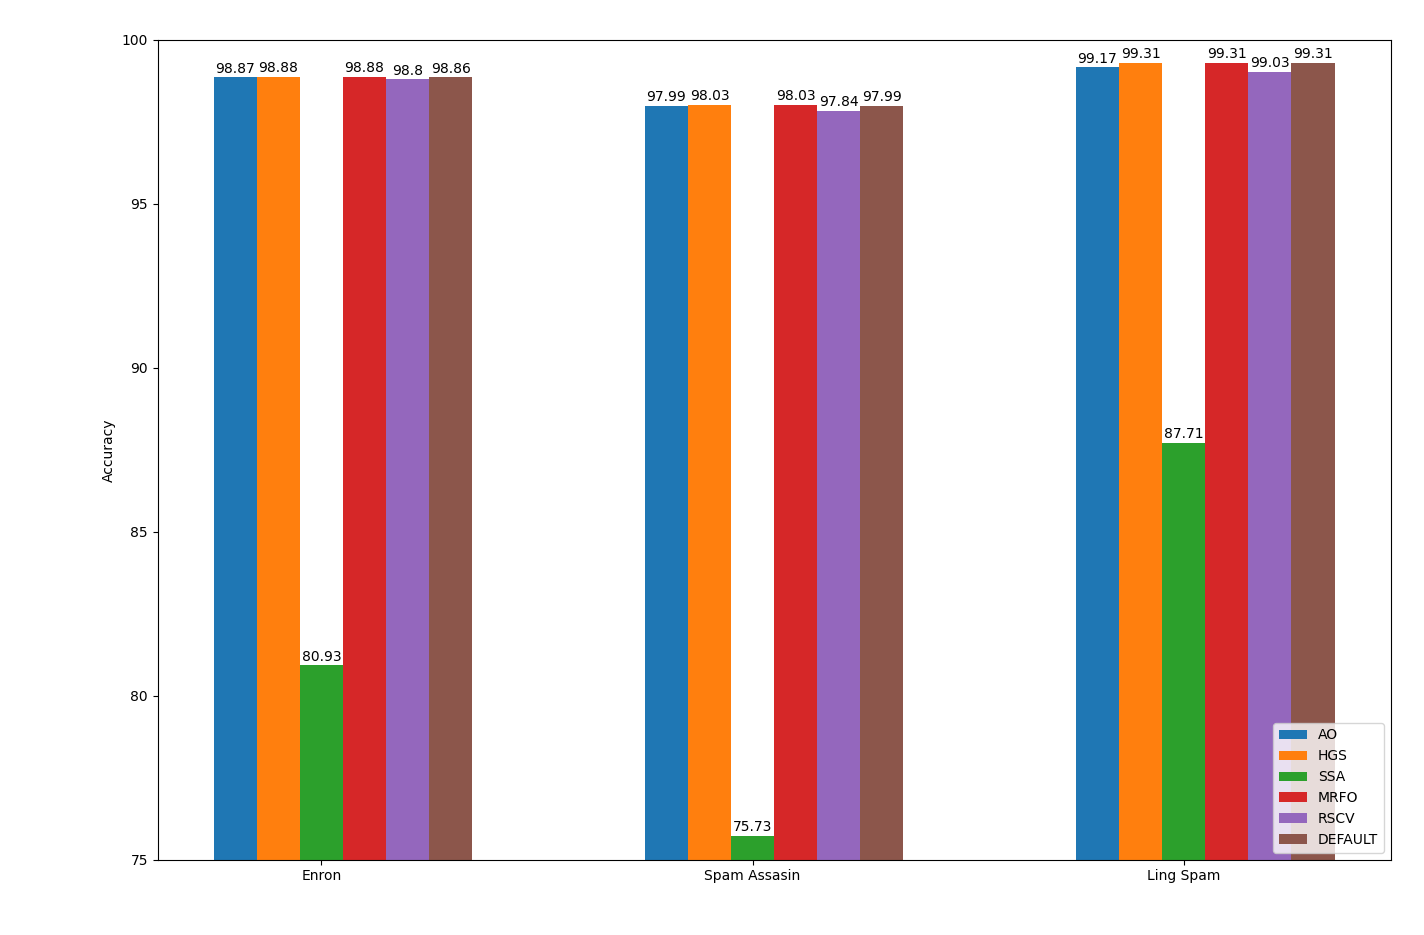
\includegraphics[width=165mm]{static/Accuracy.png}
    \caption{Accuracy для возможных сочетаний наборов данных и алгоритмов оптимизации}
    \label{AccuracyScheme}
\end{figure}

\begin{figure}[H]
    \centering
    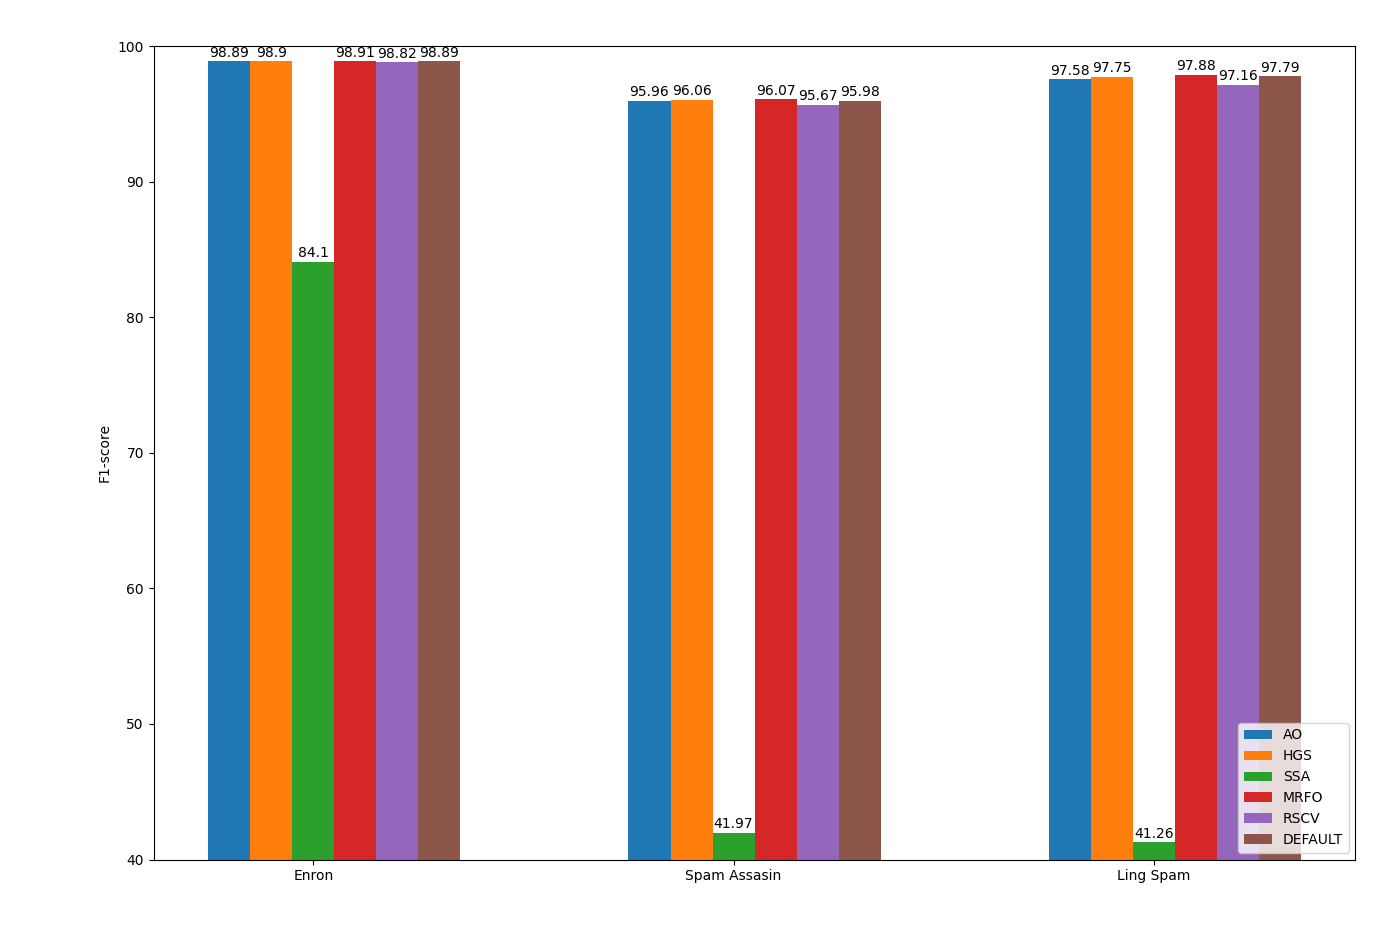
\includegraphics[width=165mm]{static/F1.png}
    \caption{F1-score для возможных сочетаний наборов данных и алгоритмов оптимизации}
    \label{F1Scheme}
\end{figure}

Анализируя результаты, можно сделать следующие выводы:

\begin{itemize}
    \item[—] Влияние настройки параметров на эффективность алгоритмов более заметно на меньших объемах данных;
    \item[—] Большее улучшение производительности по метрикам $Accuracy$ и $F1$ на всех трех наборах данных дал 
    алгоритм оптимизации кормодобывания скатов манта (MRFO);
    \item[—] Немного ниже показатели у алгоритма поиска голодных игр (HGS);
    \item[—] Алгоритм поиска воробьев (SSA), судя по показателям, оказался неподходящим для решения данной задачи;
    \item[—] Все алгоритмы оптимизации, за исключением SSA, показали результат лучше, чем случайный поиск (RSCV);
    \item[—] Параметры, выбранные алгоритмами HGS и MRFO, по сравнению с 
    параметрами по умолчанию, показали либо такие же, либо на десятые доли процента более высокие показатели производительности.
\end{itemize}


% — Программный комплекс для проведения экспериментов 
% — Набор экспериментальных метрик для каждого алгоритма, на основе которых можно выявить наиболее эффективный из предложенных алгоритмов
% — Выводы из сравнения алгоритмов
